\section{GNN}
Given the use of a graph observation, we needed a mechanism to normalize it in order to then feed it to the reinforcement learning algorithm. GNN are typically used to create an embedded representation of node features, which is then used for another task, like classification or regression. \\ \\

\noindent
Specifically, we wanted to fully take advantage of the connections between the nodes, so that every node's representation, after being processed by the GNN, would in fact include data about the neighborhood. Thus, we employed \textbf{Graph Convolutional Networks}, as described in \cite{gcn}: GCN perform a convolution on graph features, by using an update rule 
$$H^{(l + 1)} = \sigma(D^{\frac{-1}{2}} A' D^{\frac{-1}{2}} H^{l} W )$$ that, at each layer, effectively combines together features of neighboring nodes.\\ $H^0$ is the input feature matrix that contains features for each node, $W$ is a layer-specific weight matrix, while the \textbf{adjacency matrix} $A$ is actually summed with the idendity matrix in order to obtain $A'$, which considers also self-connections in the graph, otherwise each node in the GCN's output would never include information about themselves. \\
Furthermore, the \textbf{degree matrix} $D$ is included for \textit{symmetric normalization}, since the matrix multiplication risks scaling up the features.\\
Everything is then passed to an non-linear activation function $\sigma$, and repeated for a number of convolution layers which is a specific parameter of the model.\\ \\

\begin{figure}[H] 
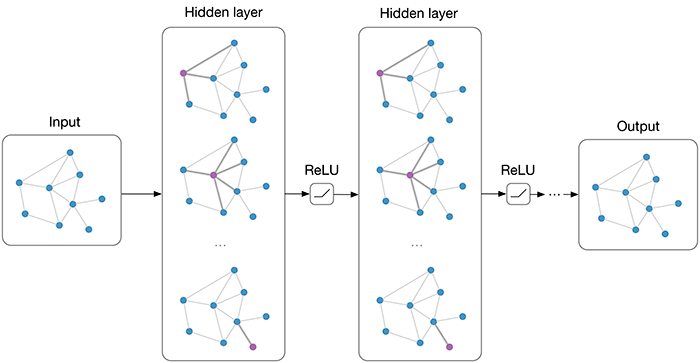
\includegraphics[height=80mm, width=140mm, scale=0.5]{chapters/gcn.png}
\centering
\caption{GCN}
\label{fig:s5} 
\end{figure}
\noindent
As features, each node has the total \textbf{distance} from every adjacent switch in the graph observation, and a one-hot encoding of its type (starting or target node, conflict, deadlock, starvation node, or other). \\
After the input node features have been processed by the gcn, agent-specific features are added to the vector representation that is then passed to the dqn.
